\documentclass[11pt,a4paper]{article}
\usepackage[utf8]{inputenc}
\usepackage[T1]{fontenc}
\usepackage[french]{babel}
\usepackage{geometry}
\usepackage{booktabs}
\usepackage{graphicx}
\usepackage{hyperref}
\geometry{margin=2.5cm}

\title{RAG Text-to-SQL pour entrepots de donnees\\
\large Recuperation conjointe du schema et de la connaissance metier}
\author{[Etudiant A] \and [Etudiant B]\\ Encadrant : [Nom]}
\date{[Annee universitaire]}

\begin{document}
\maketitle

\begin{abstract}
Ce rapport evalue un prototype Text-to-SQL qui combine retrieval de schema et
connaissance metier. Il compare quatre pipelines et teste l'hypothese H1 sur
BIRD Mini-Dev, tout en evaluant separement le retrieval documentaire sur
TPC-DS et BIRD-Evidence-Corpus. Les valeurs finales proviennent de trois
repetitions documentees dans \texttt{results/main\_study\_final}.
\end{abstract}

\section{Problematique et hypothese}
Les questions analytiques exigent a la fois des tables, colonnes et relations
correctes, ainsi que des definitions de KPI et regles metier. H1 predit une
baisse significative des erreurs semantiques du pipeline hybride D par rapport
au pipeline schema seul B, sans difference significative des erreurs
structurelles.

\section{Etat de l'art}
Le projet se positionne entre le RAG de Lewis et al., le benchmark BIRD de Li
et al. et les methodes LLM Text-to-SQL recensees par Shi et al. Contrairement
aux approches fine-tunees ou a demonstrations dynamiques, il s'agit d'un
prototype RAG modulaire par prompting. Sa contribution est experimentale :
isoler le grounding de schema du grounding metier.

\section{Protocole}
Le schema est indexe sous forme de documents table, colonnes et relations. Les
strategies BM25, embeddings et hybride sont comparees avant l'etude principale.
Sur BIRD, le champ \texttt{evidence} est injecte comme connaissance
question-specifique ; il n'est pas utilise pour revendiquer une metrique de
retrieval documentaire. Toutes les configurations principales utilisent le meme
LLM, la meme temperature et trois seeds. L'auto-correction est desactivee.

\section{Resultats}
\begin{table}[h]
\centering
\begin{tabular}{lccc}
\toprule
Pipeline & Execution Accuracy & Valid SQL Rate & Taux de refus \\
\midrule
A & $0.00\% \pm 0.00\%$ & $0.00\%$ & $79.80\%$ \\
B & $6.45\% \pm 0.00\%$ & $19.53\%$ & $71.07\%$ \\
C & $1.34\% \pm 0.10\%$ & $2.53\%$ & $42.87\%$ \\
D & $22.85\% \pm 0.19\%$ & $50.80\%$ & $22.87\%$ \\
\bottomrule
\end{tabular}
\caption{Moyenne $\pm$ ecart-type sur trois repetitions.}
\end{table}

Le pipeline hybride D obtient la meilleure Execution Accuracy et le plus fort
taux de SQL structurellement valide. L'ablation de schema retient le retrieval
hybride, avec un Table Recall@5 de $93.75\%$ et un Column Recall@5 de
$40.86\%$. Sur TPC-DS, les trois approches documentaires ont un Recall@5 de
$100\%$ sur 27 questions ; ces resultats sont separes des metriques BIRD.

\begin{figure}[h]
\centering
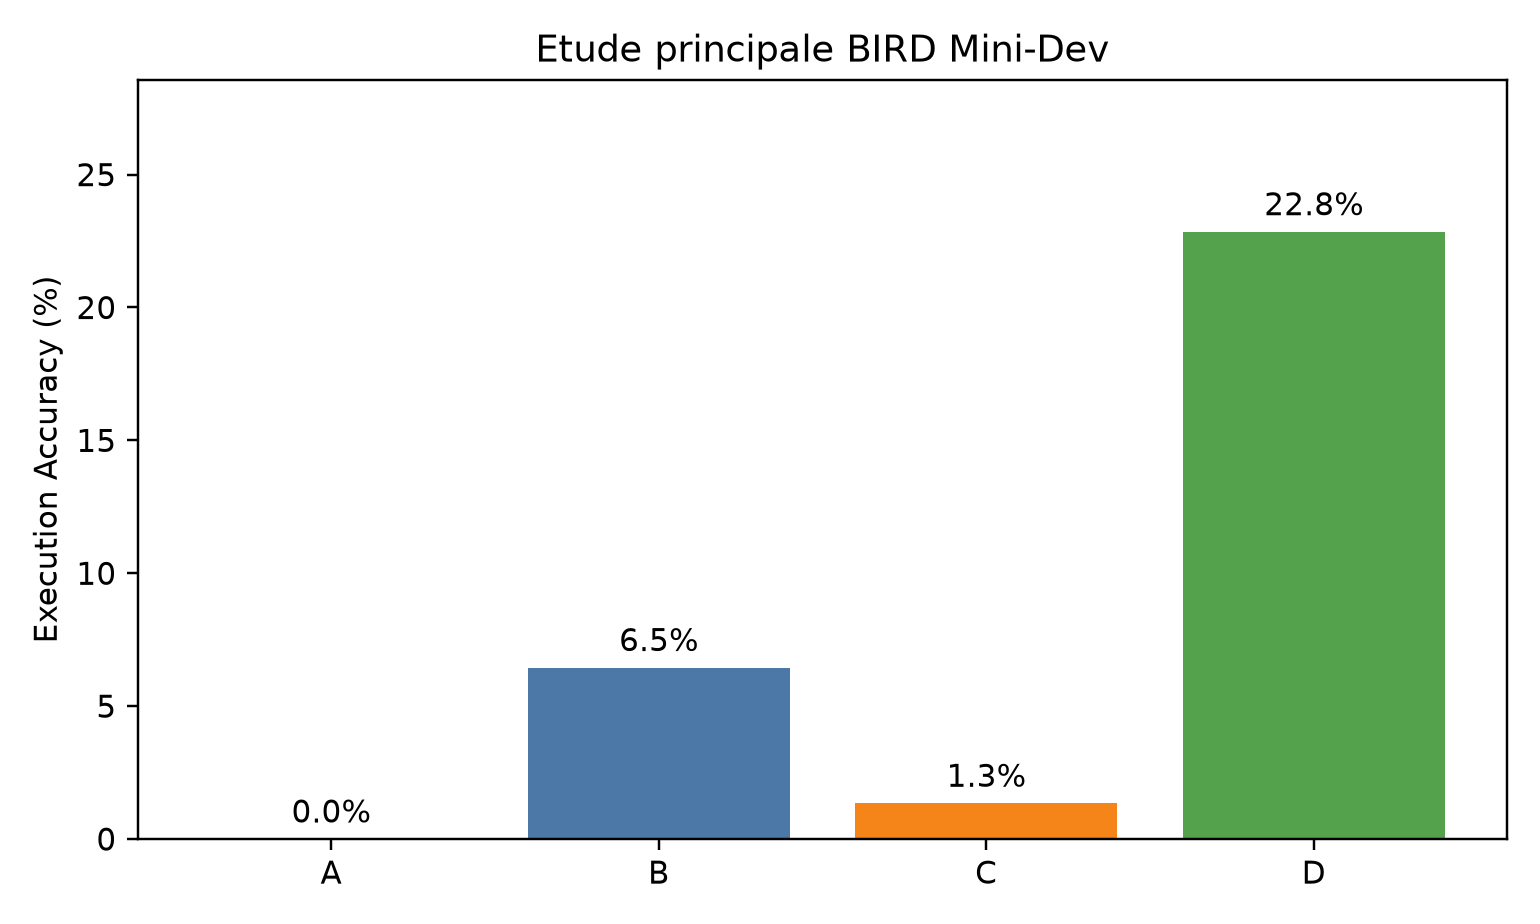
\includegraphics[width=0.72\linewidth]{../results/main_study_final/analysis/figures/execution_accuracy_by_pipeline.png}
\caption{Execution Accuracy moyenne sur les trois repetitions.}
\end{figure}

\section{Test H1 et analyse d'erreurs}
Le test est apparié : seules les questions tentees par B et D sont comparees.
McNemar exact est applique separement aux erreurs structurelles et semantiques.
Les trois runs montrent une baisse significative des erreurs semantiques :
B passe de 53.2--53.7\% a 26.1--27.2\% pour D, avec $p < 1.1\times10^{-7}$
dans chaque test exact de McNemar. Les differences structurelles ne sont pas
significatives run par run ($p=0.090$, $0.163$ et $0.121$). Le resume pooled
des paires question-run, descriptif car les questions sont repetees entre
seeds, suggere toutefois une hausse structurelle pour D ; il ne faut donc pas
revendiquer une amelioration structurelle.

Soixante cas B/D ont ete annotes. L'accord brut rapporte est de $100\%$ et
Cohen's kappa vaut $1.000$, sans desaccord. Cette valeur est interpretable
uniquement si les deux colonnes ont ete remplies independamment.

\section{Conclusion et limites}
Les resultats soutiennent une reduction robuste des erreurs semantiques par le
pipeline hybride D et une nette amelioration de l'Execution Accuracy. Ils ne
permettent pas d'affirmer une amelioration des erreurs structurelles. Une
requete executable mais fausse peut relever d'une regle metier ou d'une
jointure incorrecte ; l'annotation humaine reste donc indispensable. Les
travaux futurs couvrent le grounding sur les valeurs de base, les
demonstrations dynamiques et la correction guidee par execution.

\begin{thebibliography}{9}
\bibitem{lewis} Lewis et al. Retrieval-Augmented Generation for Knowledge-Intensive NLP Tasks. NeurIPS, 2020.
\bibitem{bird} Li et al. Can LLM Already Serve as A Database Interface? BIRD. NeurIPS, 2023.
\bibitem{survey} Shi et al. A Survey on Employing Large Language Models for Text-to-SQL Tasks. ACM CSUR, 2025.
\end{thebibliography}
\end{document}
